\documentclass[acmsmall,screen]{acmart}

\usepackage{tabularx}
\usepackage{bbm}
\usepackage{bbold}
\usepackage{stmaryrd}
\usepackage{mathpartir}
\usepackage{subcaption}
\usepackage{tikz-cd}
\usepackage{xspace}

\settopmatter{printacmref=false}
\citestyle{acmauthoryear}
\raggedbottom

\usepackage[commandnameprefix=ifneeded,commentmarkup=footnote]{changes}
\usepackage{changebar}
\input{macros}

\newcommand{\jform}[1]{\fcolorbox{black!30}{black!8}{$#1$}}
\newcommand{\Pos}{\mathsf{Pos}}

\begin{document}

\title{Inductive Types from Polynomial Endofunctors}

\maketitle

\section{Inductive types from polynomial endofunctors}
\label{sec:polynomial-types}

This section follows \citet{nunes2023}'s presentation, restricted to inductive types. Types are kinded
over a context $\Delta = \alpha_1 : \mathsf{type}, \ldots, \alpha_n : \mathsf{type}$, with $\mu\alpha.\tau$
binding a type variable in its body. Strict positivity is enforced by the kinding rule for function space:
both argument and result must be closed (kinded in the empty context), so type variables cannot occur under
$\tyFun$. A type with free kinding-context variables thus acts as a \emph{schema}: $\mu\alpha.\,\tyUnit
\tySum (\gamma \tyProd \alpha)$, kinded under $\gamma : \mathsf{type}$, becomes a particular list type by
substituting a closed type for $\gamma$. As in \citet{nunes2023}, the term language has no $\Lambda\alpha.\,
t$ or $t[\tau]$, so this is type-level parameterisation only, not parametric polymorphism.
\figref{polynomial-types:syntax} gives the syntax of types and terms.

\begin{figure}
\[
\begin{array}{rclr}
   \Delta &::=& \cdot \mid \Delta, \alpha : \mathsf{type} & \text{(kinding contexts)} \\
   \tau, \sigma &::=& \alpha \mid \tyUnit \mid \rho \mid \sigma \tySum \tau \mid \sigma \tyProd \tau \mid
                      \sigma \tyFun \tau \mid \mu\alpha.\tau & \text{(types)} \\
   t, s &::=& \cdots \mid \tmRoll{t} \mid \syn{fold}\,t\,\syn{with}\,x.s & \text{(terms)}
\end{array}
\]
\caption{Syntax of polynomial types and terms}
\label{fig:polynomial-types:syntax}
\end{figure}

\subsection{Kinding rules}
\label{sec:polynomial-types:kinding}

A type $\tau$ is \emph{well-kinded} in context $\Delta$, written $\Delta \vdash \tau : \mathsf{type}$, by
the rules in \figref{polynomial-types:kinding}. The function-space rule requires both $\sigma$ and $\tau$ to
be kinded in the empty context, so function types are closed; this rules out any occurrence of a type
variable under $\tyFun$, which suffices for strict positivity of $\mu\alpha.\tau$. The restriction is
strictly stronger than classical strict positivity (which forbids type variables only in the \emph{domain}
of $\tyFun$): our rule also excludes them from the codomain, so types like $\mu\alpha.\,\gamma \tyFun \alpha$
are ruled out even though they are strictly positive in $\alpha$. The trade-off is a rule that needs no
polarity tracking.

\begin{figure}
\begin{mathpar}
\inferrule*
  {\alpha : \mathsf{type} \in \Delta}
  {\Delta \vdash \alpha : \mathsf{type}}
\and
\inferrule*
  { }
  {\Delta \vdash \tyUnit : \mathsf{type}}
\and
\inferrule*
  {\rho \in \PrimTy}
  {\Delta \vdash \rho : \mathsf{type}}
\and
\inferrule*
  {\Delta \vdash \sigma : \mathsf{type} \\ \Delta \vdash \tau : \mathsf{type}}
  {\Delta \vdash \sigma \tyProd \tau : \mathsf{type}}
\and
\inferrule*
  {\Delta \vdash \sigma : \mathsf{type} \\ \Delta \vdash \tau : \mathsf{type}}
  {\Delta \vdash \sigma \tySum \tau : \mathsf{type}}
\and
\inferrule*
  {\cdot \vdash \sigma : \mathsf{type} \\ \cdot \vdash \tau : \mathsf{type}}
  {\Delta \vdash \sigma \tyFun \tau : \mathsf{type}}
\and
\inferrule*
  {\Delta, \alpha : \mathsf{type} \vdash \tau : \mathsf{type}}
  {\Delta \vdash \mu\alpha.\tau : \mathsf{type}}
\end{mathpar}
\caption{Kinding rules for types}
\label{fig:polynomial-types:kinding}
\end{figure}

\subsection{Syntactic polynomials}
\label{sec:polynomial-types:poly}

Let $\cat{C}$ be a category with finite products $(\times, \One)$ and finite coproducts
$(\coprod, 0)$. The \emph{polynomials} over $\cat{C}$ are functor expressions in a kinding context
$\Delta$:
\[
  P, Q \in \Poly_\Delta \;::=\; \const(A) \mid \alpha \mid P + Q \mid P \times Q \mid \mu\alpha.P
\]
where $A$ ranges over objects of $\cat{C}$ and $\alpha$ over the variables of $\Delta$.
Polynomials mirror the types of \secref{polynomial-types:kinding}, with constants in place of primitive
types. Function space is absent because function types are closed (\figref{polynomial-types:kinding}),
so a function type denotes a fixed object and enters a polynomial as a constant. We identify each $P
\in \Poly_\Delta$ with the functor $\cat{C}^\Delta \to \cat{C}$ it presents, writing $P(\delta)$ for
its action on a \emph{kinding environment} $\delta \in \cat{C}^\Delta$, an assignment of an object to
each variable of $\Delta$; the $\mu$ clause presupposes initial algebras, supplied as structure on
$\cat{C}$ by \defref{polynomial-types:has-poly} below. Presenting functors by a syntax of signatures,
interpreted afterwards, is standard in the literature on containers and strictly positive types
\citep{abbott2005}; \citet{gambino-kock} treat polynomial functors as a categorical subject in their
own right.

\citet[Definition~6]{nunes2023} instead define the polynomial endofunctors on $\cat{C}$
semantically, as the smallest subcategory of $\Cat$ containing the product and coproduct functors,
projections, pairing and constants, and closed under forming $\mu H$ whenever it exists. An expression
of type $\Poly_\Delta$ is in effect a derivation of membership in this class, detached from its side
conditions, so it exists whether or not the initial algebras do. The construction of
\secref{polynomial-types:fam} recurses on the expression to establish that the initial algebras exist,
and, by substituting at the constants, interprets the same expression in both $\Fam(\cat{C})$ and sets.

\subsection{Typing rules}
\label{sec:polynomial-types:language}

Typing contexts $\Gamma = x_1 : \sigma_1, \ldots, x_n : \sigma_n$ have all $\sigma_i$ closed
($\cdot \vdash \sigma_i : \mathsf{type}$). The typing rules for $\syn{roll}$ and $\syn{fold}$ are
\begin{mathpar}
\inferrule*
  {\Gamma \vdash t : \subst{\tau}{\mu\alpha.\tau}{\alpha}}
  {\Gamma \vdash \tmRoll{t} : \mu\alpha.\tau}
\and
\inferrule*
  {\Gamma \vdash t : \mu\alpha.\tau \\
   \Gamma, x : \subst{\tau}{\sigma}{\alpha} \vdash s : \sigma}
  {\Gamma \vdash \syn{fold}\,t\,\syn{with}\,x.s : \sigma}
\end{mathpar}
with $\sigma$ closed and $\tau$ kinded in context $\alpha : \mathsf{type}$. The $\fold$ rule uses the
parametric (open) form of the catamorphism: the fold body $s$ lives in the extended context $\Gamma, x :
\subst{\tau}{\sigma}{\alpha}$ rather than as a closed function, avoiding the need for exponentials in the
semantic category.

\subsection{Existence of initial algebras in $\Fam(\cat{C})$}
\label{sec:polynomial-types:fam}

\citet[Proposition~81]{nunes2023} establish that $\Fam(\Set)$ has initial algebras for their polynomials. We
give a direct construction in $\Fam(\cat{C})$ via Martin-L\"of $W$-types
\citep[Wellorderings, pp.~43--47]{martinLof1984}, restricted to the finitary fragment (where each shape has
finite arity), which suffices because our polynomials are built from finite $+$ and $\times$.
\citet{moerdijk-palmgren00} study $W$-types categorically, as initial algebras of polynomial
endofunctors.

We take polynomials (\secref{polynomial-types:poly}) over $\Fam(\cat{C})$, so each constant
$\const(A)$ carries a family $A = (X, \partial X)$.

The fold body of the $\syn{fold}$ rule of \secref{polynomial-types:language} lives in a typing context,
so the catamorphism interpreting it must too. A \emph{morphism in context $\Gamma$} from $X$ to $Y$ is
a map $\Gamma \times X \to Y$, composed by $f \circ_\Gamma g = f \circ \prodM{\pi_1}{g}$; these are
the maps of the co-Kleisli category for the comonad $\Gamma \times -$. Each polynomial acts on
morphisms in context through the \emph{strong} functorial action, which takes a morphism in context
$\Gamma \times X_i \to Y_i$ for each variable $i$. Below, $F = P(\delta[\alpha \mapsto -])$.

\begin{definition}[$\Poly$-types]
\label{def:polynomial-types:has-poly}
A category \emph{has $\Poly$-types} if for each $P \in \Poly_{\Delta,\alpha}$ and kinding environment $\delta$
it provides:
\begin{itemize}
\item an object $\mu_{\alpha.P}(\delta)$ and algebra map $\inMap : P(\delta[\alpha \mapsto
  \mu_{\alpha.P}(\delta)]) \to \mu_{\alpha.P}(\delta)$;
\item for every $\Gamma$ and algebra $a : \Gamma \times P(\delta[\alpha \mapsto Y]) \to Y$, a map
  $\cata{a} : \Gamma \times \mu_{\alpha.P}(\delta) \to Y$, its \emph{catamorphism}, the unique
  morphism in context making
  \begin{center}
  \begin{tikzcd}[row sep=2.2em, column sep=3.2em]
    F\,\mu_{\alpha.P}(\delta) \arrow[r, "\inMap"] \arrow[d, dashed, "F\cata{a}"'] &
      \mu_{\alpha.P}(\delta) \arrow[d, dashed, "\cata{a}"] \\
    F\,Y \arrow[r, "a"'] & Y
  \end{tikzcd}
  \end{center}
  commute in the co-Kleisli category: commutation of the square is the law $\beta$, and uniqueness
  of $\cata{a}$ the law $\eta$.
\end{itemize}
\end{definition}

\noindent
Unfolding $\circ_\Gamma$, the initiality square commutes in the underlying category as
\begin{center}
\begin{tikzcd}[row sep=2.4em, column sep=5em]
  \Gamma \times F\,\mu_{\alpha.P}(\delta) \arrow[r, "\id \times \inMap"]
    \arrow[d, "{\prodM{\pi_1}{F\cata{a}}}"'] &
    \Gamma \times \mu_{\alpha.P}(\delta) \arrow[d, "\cata{a}"] \\
  \Gamma \times F\,Y \arrow[r, "a"'] & Y
\end{tikzcd}
\end{center}
\noindent
where the left edge duplicates the context, retaining $\Gamma$ for $a$ while also feeding it
to the strong action $F\cata{a}$. In element notation, for the polynomial $\const(A) \times \alpha$
the strong action sends $h : \Gamma \times X \to Y$ to $(\gamma, (a, x)) \mapsto (a, h(\gamma, x))$:
the context reaches each variable position, and constants pass through.

Taking $\Gamma = 1$, each $\mu_{\alpha.P}(\delta)$ is in particular an initial algebra in the usual
sense; in the presence of exponentials the strong form is no extra imposition (fold into $Y^\Gamma$), but
$\Fam(\cat{C})$ need not have exponentials. Initial algebras equipped with catamorphisms in
context are the strong datatypes of \citet{cockett-spencer92}, developed for categories with finite
products but not necessarily exponentials. \citet[Definition~6]{nunes2023} accordingly ask only for
initial algebras, their semantic categories being bicartesian closed. At the term level, $\beta$ reduces
$\syn{fold}\,(\syn{roll}\,t)\,\syn{with}\,x.s$ by recursively folding each $\mu$-child of $t$ before
substituting into $s$, and $\eta$ says $\syn{fold}\,t\,\syn{with}\,x.\syn{roll}\,x = t$.

\begin{proposition}
\label{prop:polynomial-types:fam-has-poly}
If $\cat{C}$ has finite products $(\times, 1)$ then $\Fam(\cat{C})$ has $\Poly$-types.
\end{proposition}

The proof builds the initial algebras directly, and runs to the end of the subsection; the
definitions below supply its carrier and the fibres over it. Nested $\mu$s make the naive
construction circular: when an inner binder's body mentions an outer binder,
the inner carrier must be instantiated at the outer carrier while the latter is still being defined.
Following \citet{abbott2004} we instead construct the initial algebras of $P$ and of all its inner
$\mu$-bodies simultaneously, as a single family of trees indexed by sorts.

The construction separates into two layers, and the first uses index data only. The separation
is possible because $\Fam(\cat{C})$ is the free coproduct completion of $\cat{C}$, so an object is a
set-indexed collection of $\cat{C}$-objects and nothing more. Write $|A|$ for the
index set of a $\Fam(\cat{C})$-object $A$.

\begin{definition}[Index erasure]
\label{def:polynomial-types:erasure}
The \emph{index erasure} $|Q|$ of a polynomial $Q$ over $\Fam(\cat{C})$ replaces each constant
$\const(X, \partial X)$ by $\const(X)$ and keeps the rest unchanged, giving a polynomial over
$\Set$. The index erasure $|\delta|$ of a kinding
environment $\delta \in \Fam(\cat{C})^\Delta$ replaces each entry by its index set, giving $|\delta|
\in \Set^\Delta$.
\end{definition}

The sorts and trees below are defined over $|Q|$ and $|\delta|$, so they make no reference to
$\cat{C}$. The fibres form the second layer, assigning to each tree an object of $\cat{C}$. Two
presentations agreeing on all index sets, even over different categories, therefore determine the
same sorts and trees.

\begin{definition}[Sort]
\label{def:polynomial-types:sort}
A \emph{sort} $\sigma = (\alpha.R, \rho)$ over $\Delta$ is a pair of an \emph{abstraction}
$\alpha.R$, an index-erased polynomial $R$ with a distinguished \emph{recursion variable} $\alpha$,
and an \emph{assignment} $\rho$ taking each other free variable of $R$ to a parameter in $\Delta$ or
another sort.
\end{definition}

Since an assignment may send a variable to another sort, this definition is inductive.

\begin{definition}[Trees of a sort]
\label{def:polynomial-types:trees}
Work over the erased environment $|\delta|$. For each sort $(\alpha.R, \rho)$ the set
$W_{(\alpha.R,\rho)}$ of \emph{trees of sort $(\alpha.R, \rho)$}, and for each index-erased
polynomial $R'$ with an assignment $\rho'$ of its variables the set of \emph{$R'$-trees}, are
defined by a single simultaneous induction \citep{abbott2004}:
\begin{itemize}
\item a tree of sort $(\alpha.R, \rho)$ is an $R$-tree, the recursion variable $\alpha$ assigned the
  sort $(\alpha.R, \rho)$ itself;
\item a $\const X$-tree is an element of $X$;
\item a $\beta$-tree is an element of $|\delta|(\rho'(\beta))$ if $\rho'(\beta)$ is a parameter, and a
  tree of sort $\rho'(\beta)$ otherwise;
\item a $(R_1 + R_2)$-tree is an $R_1$-tree or an $R_2$-tree, tagged with the summand;
\item a $(R_1 \times R_2)$-tree is a pair of an $R_1$-tree and an $R_2$-tree;
\item a $\mu\beta.R'$-tree is a tree of sort $(\beta.R', \rho')$.
\end{itemize}
\end{definition}

\begin{definition}[Decoration]
\label{def:polynomial-types:decoration}
A \emph{decoration} of a sort $(\alpha.R, \rho)$ is a polynomial $Q$ over $\Fam(\cat{C})$ with $|Q| =
R$, together with a decoration of each sort in the range of $\rho$. Decorations are data over the
sorts, so the trees do not depend on them, and a decoration determines the sort it decorates. The
root sort is decorated by $P$ itself, and a decoration induces decorations of the sorts reachable
from its sort, each inner $\mu$-body decorating the sort it erases to.
\end{definition}

\begin{definition}[Fibres]
\label{def:polynomial-types:fibres}
For a decorated sort $\sigma$, the \emph{fibre} $\partial W_\sigma(t) \in \cat{C}$ of a tree $t \in
W_\sigma$ recovers the erased objects, by structural recursion on $t$:
\begin{itemize}
\item the fibre of a tree of sort $(\alpha.R, \rho)$ is the fibre of the underlying $R$-tree;
\item the fibre of a $\const X$-tree $x$ is $\partial X_x$, where $\const(X, \partial X)$ is the
  constant supplied by the decoration;
\item the fibre of a $\beta$-tree is the corresponding fibre of $\delta(\rho'(\beta))$ if
  $\rho'(\beta)$ is a parameter, and the fibre of the tree of sort $\rho'(\beta)$ otherwise;
\item the fibre of a $(R_1 + R_2)$-tree is the fibre of the underlying $R_i$-tree;
\item the fibre of a $(R_1 \times R_2)$-tree is the product of the fibres of its components;
\item the fibre of a $\mu\beta.R'$-tree is the fibre of the underlying tree of sort $(\beta.R',
  \rho')$, decorated by the corresponding $\mu$-body of the decoration.
\end{itemize}
\end{definition}

\paragraph{Worked example: rose trees.}
Take $P = \const(A) \times \mu\beta.(\const(\One_{\!F}) + \alpha \times \beta) \in
\Poly_{\alpha}$ over $\Fam(\cat{C})$, where $A = (|A|, \partial A)$ is a family and $\One_{\!F}$ the
terminal family (one index, terminal fibre): a rose tree carries an $A$-label and a list of subtrees.
The inner body mentions the outer variable $\alpha$, so
the naive construction is circular, because the list carrier must be instantiated at $\mu_{\alpha.P}$
while the latter is still being defined. $P$ has two sorts (\defref{polynomial-types:sort}),
\[
  s_0 = \bigl(\alpha.(|A| \times \mu\beta.(1 + \alpha \times \beta)),\; \cdot\,\bigr) \qquad
  s_1 = \bigl(\beta.(1 + \alpha \times \beta),\; \alpha \mapsto s_0\bigr)
\]
the root sort and the sort of the inner $\mu$-body. Each sort's own recursion variable ($\alpha$
in $s_0$, $\beta$ in $s_1$) refers to that sort itself; the entry $\alpha \mapsto s_0$ of $s_1$
records symbolically that the inner body uses the outer binder, with no need for the outer carrier
to exist yet. By \defref{polynomial-types:trees}, a tree of sort $s_0$ is an element of $|A|$ paired
with a tree of sort $s_1$, and a tree of sort $s_1$ is either the left tag (end of list) or a tree
of sort $s_0$ paired with a further tree of sort $s_1$. So $W_{s_0}$ contains exactly the
$|A|$-labelled rose trees and $W_{s_1}$ their forests, generated by one simultaneous induction.
Decorating $s_0$ by $P$
(\defref{polynomial-types:decoration}) restores the fibres $\partial A$ that erasure forgot, and the
fibre of a tree (\defref{polynomial-types:fibres}) multiplies them over its nodes:
\begin{center}
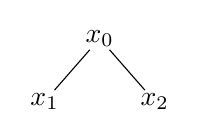
\begin{tikzpicture}[level distance=8mm, sibling distance=14mm, every node/.style={inner sep=1pt}]
\node {$x_0$} child {node {$x_1$}} child {node {$x_2$}};
\end{tikzpicture}
\qquad\raisebox{5.5mm}{$\partial W_{s_0} = \partial A_{x_0} \times \bigl((\partial A_{x_1} \times 1)
  \times ((\partial A_{x_2} \times 1) \times 1)\bigr) \;\cong\; \partial A_{x_0} \times \partial
  A_{x_1} \times \partial A_{x_2}$}
\end{center}
\noindent
where the units come from the list ends and the leaves' empty forests. The proposition's
carrier $(W_{s_0}, \partial W_{s_0})$ is therefore the family of rose trees with, over each tree,
the product of its label fibres; the algebra map builds a tree from a label and a forest, and on
fibres it is the identity, both sides being the same node-wise product.

\begin{proof}[Proof of \propref{polynomial-types:fam-has-poly}]
Take $\mu_{\alpha.P}(\delta) = (W_{s_0}, \partial W_{s_0})$, the family at the root sort $s_0 =
(\alpha.|P|, \rho_0)$ decorated by $P$, where $\rho_0$ takes the free variables of $P$ to the
parameters $\Delta$. The sorts arising are those reachable from $s_0$, following the sort assigned at
each nested $\mu$.

For the algebra map $\inMap : P(\delta[\alpha \mapsto \mu_{\alpha.P}(\delta)]) \to
\mu_{\alpha.P}(\delta)$, compute the domain by induction on $P$. An element of its index set is the
tuple of arguments to one application of the tree constructor: a label at each constant, a tag at each sum,
a pair at each product, an $s_0$-subtree at each occurrence of $\alpha$, and at each inner
$\mu$-body a subtree of its sort in which the $\alpha$-positions again hold $s_0$-subtrees.
\defref{polynomial-types:trees} admits exactly these arguments under the root of an $s_0$-tree, so
on index sets $\inMap$ forms the tree with the arguments beneath a new root node, invertibly,
decomposition at the root being its inverse; in the rose-tree example
\begin{center}
$\inMap : \bigl(x_0,\ [\,T_1,\ T_2\,]\bigr) \;\longmapsto\;$
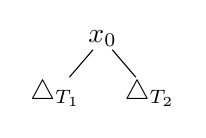
\begin{tikzpicture}[baseline=-8mm, level distance=7mm, sibling distance=12mm,
                    every node/.style={inner sep=1pt}]
\node {$x_0$} child {node {$\triangle_{T_1}$}} child {node {$\triangle_{T_2}$}};
\end{tikzpicture}
\end{center}
\noindent
with the triangles standing for the subtrees $T_1$ and $T_2$. On fibres $\inMap$ is the identity,
because \defref{polynomial-types:fibres} computes the fibre of the new tree by the same product
structure that the action of $P$ computes on the arguments; in the example, both sides are the same
node-wise product of label fibres.

For an algebra $a : \Gamma \times P(\delta[\alpha \mapsto Y]) \to Y$, the catamorphism
$\cata{a} : \Gamma \times \mu_{\alpha.P}(\delta) \to Y$ is defined by structural recursion over
trees, simultaneously over all sorts, threading the $\Gamma$-component unchanged. In the rose-tree
example, on index sets,
\[
  \cata{a}\bigl(\gamma,\ \inMap(x_0,\ [\,T_1,\ T_2\,])\bigr) \;=\;
  a\bigl(\gamma,\ (x_0,\ [\,\cata{a}(\gamma, T_1),\ \cata{a}(\gamma, T_2)\,])\bigr).
\]
\noindent
In general, the root is decomposed into its arguments, the recursion is applied to each
$s_0$-subtree, and $a$ combines the results. At an inner sort the recursion translates its trees from
the environment $\delta$ to the environment $\delta[\alpha \mapsto Y]$ by the strong action,
replacing each $s_0$-subtree by its folded value and leaving the surrounding structure intact (the
list over $Y$ in the equation above), so that the translated arguments land in the domain of $a$. The
same recursion is performed on fibres.

The law $\beta$ is the unfolded initiality square of \defref{polynomial-types:has-poly},
taken at the concrete carriers. The upper path forms the tree with the arguments as its immediate
subtrees and then folds it; the lower path folds the $s_0$-subtrees inside the arguments and then
applies $a$. Both compute the same recursion on trees, and the equation above is $\beta$ at the
example. For $\eta$, let $h$ satisfy $\beta$ in place of $\cata{a}$; by induction on trees
(simultaneously over all sorts), $h$ agrees with $\cata{a}$ at every tree, the inductive
hypothesis covering the $s_0$-subtrees among the arguments.
\end{proof}

\subsection{The $\mu$-operator}
\label{sec:polynomial-types:mu-operator}

The construction of \secref{polynomial-types:fam} is pointwise in the kinding environment
$\delta$. This subsection derives the remaining structure, the action of $\mu_{\alpha.P}$ on morphisms
of environments and its laws, from $\beta$ and $\eta$ alone, so everything here holds in any category
with $\Poly$-types, independently of the construction. Fix $P \in \Poly_{\Delta,\alpha}$, write
$\inMap_\delta$ for the algebra map at $\delta$, and $F = P(\delta[\alpha \mapsto -])$. All diagrams
are squares of morphisms in context $\Gamma$, composed by $\circ_\Gamma$.

As in \citet[Proposition~4]{nunes2023}, the action on a morphism $g : \delta \to \delta'$ is
given by folding: $\mu_{\alpha.P}(g) = \cata{\,\inMap_{\delta'} \circ P(g[\alpha \mapsto \id])\,}$,
the algebra built from the strong action of $P$. By $\beta$ and $\eta$, $\mu_{\alpha.P}(g)$ is the
unique map making
\begin{center}
\begin{tikzcd}[row sep=2.2em, column sep=5em]
  P(\delta[\alpha \mapsto \mu_{\alpha.P}(\delta)]) \arrow[r, "\inMap_\delta"]
    \arrow[d, "{P(g[\alpha \mapsto \mu_{\alpha.P}(g)])}"'] &
    \mu_{\alpha.P}(\delta) \arrow[d, "\mu_{\alpha.P}(g)"] \\
  P(\delta'[\alpha \mapsto \mu_{\alpha.P}(\delta')]) \arrow[r, "\inMap_{\delta'}"'] &
    \mu_{\alpha.P}(\delta')
\end{tikzcd}
\end{center}
commute: the algebra maps are natural in the environment.

The laws of this action follow from one standard consequence of initiality.

\begin{lemma}[Fusion]
\label{lem:polynomial-types:fusion}
Let $a : \Gamma \times FY \to Y$ and $b : \Gamma \times FZ \to Z$ be algebras and $h : \Gamma \times
Y \to Z$. If $h \circ_\Gamma a = b \circ_\Gamma Fh$ then $h \circ_\Gamma \cata{a} = \cata{b}$.
\end{lemma}
\begin{center}
\begin{tikzcd}[row sep=2.2em, column sep=3.2em]
  F\,\mu_{\alpha.P}(\delta) \arrow[r, "\inMap_\delta"] \arrow[d, "F\cata{a}"'] &
    \mu_{\alpha.P}(\delta) \arrow[d, "\cata{a}"] \\
  F\,Y \arrow[r, "a"] \arrow[d, "Fh"'] & Y \arrow[d, "h"] \\
  F\,Z \arrow[r, "b"'] & Z
\end{tikzcd}
\end{center}
\noindent
The upper square is $\beta$; when the lower square commutes, the outer rectangle states that
$h \circ_\Gamma \cata{a}$ satisfies the $\beta$-law characterising $\cata{b}$ (this uses that $F$
preserves $\circ_\Gamma$), so the two are equal by uniqueness. Fusion gives the functor laws directly:
$\mu_{\alpha.P}(\id) = \id$ is $\eta$, and pasting the naturality square of $g$ above that of $g'$
exhibits $\mu_{\alpha.P}(g') \circ_\Gamma \mu_{\alpha.P}(g)$ as a fold of the algebra defining
$\mu_{\alpha.P}(g' \circ g)$.

Uniqueness also shows the initial algebra is determined by the polynomial up to isomorphism:
if $\varphi : P(\delta) \cong Q(\delta)$ naturally in $\delta$, the folds
$\cata{\inMap^Q \circ \varphi}$ and $\cata{\inMap^P \circ \varphi^{-1}}$ compose, by fusion, to folds
of $\inMap^P$ and $\inMap^Q$, which are identities by $\eta$; so $\mu_{\alpha.P}(\delta) \cong
\mu_{\alpha.Q}(\delta)$. The same pattern at $\Gamma = 1$ gives Lambek's lemma \citep{lambek68}:
$\inMap_\delta$ is itself an isomorphism, with inverse $\cata{F\,\inMap_\delta}$, so
$\mu_{\alpha.P}(\delta)$ is a fixed point of $F$.

The strong action makes each $P$ the morphism part of a functor $(\cat{C}_\Gamma)^\Delta \to
\cat{C}_\Gamma$ on co-Kleisli categories, the plain action being its restriction to pure morphisms
$\prodM{\pi_1}{g \circ \pi_2}$. For a $\mu$-subexpression the functoriality that fusion assumes of
$F$ is the functoriality being proved, at the inner binder; the two are established together by
induction on the polynomial expression.

\input{mu-types/conservativity}

\bibliographystyle{ACM-Reference-Format}
\bibliography{bib}

\clearpage
\appendix
\input{mu-types/no-cbn}

\end{document}
